%% LyX 2.3.4.2 created this file.  For more info, see http://www.lyx.org/.
%% Do not edit unless you really know what you are doing.
\documentclass[english]{report}
\usepackage[T1]{fontenc}
\usepackage[latin9]{inputenc}
\usepackage{amsmath}
\usepackage{graphicx}

\makeatletter
%%%%%%%%%%%%%%%%%%%%%%%%%%%%%% User specified LaTeX commands.
\usepackage{lmodern}
\usepackage{microtype}
\usepackage{textcomp}
\frenchspacing

\@ifundefined{showcaptionsetup}{}{%
 \PassOptionsToPackage{caption=false}{subfig}}
\usepackage{subfig}
\makeatother

\usepackage{babel}
\begin{document}
\title{Modeling and evaluation}

\maketitle
In the previous chapter, the coordination mechanisms developed in
\cite{Cattaneo2017} have been presented, giving particular attention
to the contribution provided by proactivity. Concerning buddy system
and reserve, their proactive versions move the idle set at the barycenter
of the positions of the active agents. This ensures good results when
compared with the base method, in particular for proactive reserve.
However, the location for the idle set is computed naively and might
be exploiting only a part of the information available at the moment
related to the structure of the environment. For example, the barycenter
of the positions of the active robots may fall into a small room,
from which a robot in the idle set would have to get off once turned
into active, making the move into the room almost useless. On the
contrary, we are more interested in moving the robots in the idle
set towards positions providing a good starting point for them. 

To include the structure of the environment directly into the coordination
mechanism, graphs are considered. They provide a representation of
the free space and computing some suitable metrics, called centrality
metrics, it is possible to find out a subset of nodes more influential
on connectivity between spaces. In this way, the proactivity location,
i.e., the location where the idle set is proactively moved, is a central
point of the environment. The concept of centrality varies accordingly
to the centrality metric used to compute such subset of nodes. In
the following, the graphs and the centrality metrics used in this
work will be presented and described in-depth. The last section is
dedicated to providing an overview of the criteria used to evaluate
the different coordination mechanisms tested.

\section{Graphs}

The use of graphs allows including a topological component in the
coordination, which is done employing an embedded graph. A graph $G$
embedded to a surface $\Sigma$ is a representation of $G$ on $\Sigma$
such that points of $\Sigma$ and arcs in it are associated with vertices
and edges of $G$ respectively. This concept is applied by creating
a graph $\varUpsilon$ embedded on the map $M$ and then through the
measures of the centrality of a node, nodes are ranked based on their
values for the two centrality measures used in this work.

The definition of an embedded graph is independent of the actual implementation
of it and this leaves the freedom to adapt the correspondence points-nodes
and arcs-edges on the needs. Based on this, two different types of
graphs are defined in the next sections. 

These graphs differ strongly on how they are defined and how they
model the environment. The first one is more focused on the topological
properties of the environment, nodes and edges are computed based
on the structure of the known free space. The model it provides is
not strictly affected by team-dependent factors like agents distribution
or team size, being built only considering the connectivity properties
of the map. On the contrary, the second kind of graph defined below
is built according to the positions of the agents moving in the environment.
In this way, it includes information related to the disposition of
the agents and the path followed. Moreover, it is also indirectly
affected by the structure of the environment, being the agents only
capable of moving in the free space, the routes they travel outline
the connectivity among the different spaces. In the following, how
frontiers are introduced into the graph building process is also explained. 

The following sections explain in detail how the two types of graphs
are built during the exploration process, starting with the topological
graph and then moving on to the visibility one. 

\subsection{Topological graph}

From now on, as \emph{topological graph} will be identified a graph
isomorphic to the graph used by the simulator to compute the path
followed by the agents during the exploration. As presented in \cite{Spirin2015},
the construction of this one is based on the structure of the occupancy
grid known up to that moment, in which the skeleton of the free space
is found by performing thinning. A discretization is then applied
to the skeleton to find the set of nodes composing the graph and nodes
linked by the skeleton are also connected by an edge, weighted according
to the distance between the nodes. This process is sufficient to provide
a simple topological graph embedded on the map of the environment. 

On one side, the use of this graph is backed up by the implementation
of the navigation system, because it is computed just once for both
the applications and in this way it does not introduce further costs
in the building and the update. On the other side, it is pretty limited
in its representation. It suffices to provide a topological view of
the environment, but it is hard to extend with elements like frontier
nodes or information about the location of the robots. Two aspects
that characterize the second kind of graph tested, the visibility
graph. 

In Figure 1.a, the topological graph of the environment presented
in the previous chapter is shown. This one has been produced by applying
the building procedure on the whole map of the environment when it
has been completely mapped. This has been considered to show more
clearly the properties of this graph. The disposition of the nodes
is almost uniform and this can be particularly noticed by looking
at their distribution in the lateral rooms. Being these spaces almost
equal in structure, nodes are placed with the same pattern. Moreover,
the distance among nodes tends to be almost the same on the entire
map, with a slight reduction at the conjunctions. This almost uniform
distribution highlights strongly the difference in structure with
the visibility graph, shown in Figure 1.b, where nodes are provided
with varying concentrations among the various spaces. 

\subsection{Visibility graph }

The \emph{visibility graph }as defined in this work consists of a
graph built on the notion of visibility, rather than the navigability
from node to node. It is composed of two different types of nodes,
the \emph{pose nodes,} and the \emph{frontier nodes}. 

The first kind is the one composing the vast majority of the graph
and each node has an historical meaning, being a pose assumed by an
active robot during the exploration. As active agents proceed in their
mapping task, their locations are stored as nodes every time a re-plan
for one of them or a new location for the robots in the idle set is
needed. These two events happen quite frequently in the initial part
of the exploration, and thus they trigger the graph building function
enough times. However, the frequency with which this is done is variable,
for this reason, the distribution of the nodes might be loose in some
spaces and more tight in others. This allows keeping the number of
nodes in the graph reduced with respect to the case in which every
time an active agent moves, its pose is used to set up a pose node.
Nevertheless, as long as connectivity is ensured, the effect on the
information obtainable by the graph is almost the same and by keeping
the size of the graph reduced, the complexity of computing centrality
measures remains manageable. To enforce this aspect, the location
of an active agent is added as a pose node as long as there are no
other pose nodes within a certain radius. Once a pose node is added
to the graph, it is fixed and never modified as the exploration goes
on. The motion of agents in the idle set is excluded to avoid an excessive
concentration of nodes in some crucial areas, which would negatively
affect the computation of centrality measures. 

The second kind of node is frontier nodes. As the name suggests, they
allow to include the frontiers computed by the exploration strategy
into the graph. This is a fundamental characterization of this graph
in the distinction from the topological one. At each step in which
the list of frontiers is updated, the same is done for the list of
frontier nodes: the old ones which have been explored are removed
and the new ones are added, making this type of nodes variable in
time differently from pose nodes which are fixed once they are put
in the graph.

An edge models the notion of visibility: two nodes $n_{1}$ and $n_{2}$
are linked by an edge if and only if $n_{1}$is within the sensing
range of a robot placed in $n_{2}$ and there are no obstacles along
the straight line connecting them. This relation holds in both the
directions, thus the visibility graph is an undirected graph by construction,
same as the topological one. Edges are also characterized by a weight
equal to the distance between the nodes.

Figure 1.b shows the visibility graph built by a team of robots during
the exploration. Accordingly to what stated previously, the distribution
of nodes depends strongly on the path followed by the robots and on
the frequency with which the graph is updated. The structural differences
with the topological graph in Figure 1.a are clean just by looking
at the two figures and all relate to the distribution of nodes, being
widely less uniform. Frontier nodes, here painted in red, are also
a discriminating factor between the two.

\begin{figure}
\subfloat[Topological graph. Green dots represent the nodes]{\includegraphics[width=6cm]{\string"/home/alex/Scrivania/desktop/Tesi/Documenti/Marco Catteneo/MRESim/logs/disegni/d3t\string".eps}

}\quad{}\subfloat[Visibility graph. Green dots represent pose nodes, red ones are the
frontier nodes ]{\includegraphics[width=6cm]{\string"/home/alex/Scrivania/desktop/Tesi/Documenti/Marco Catteneo/MRESim/logs/disegni/d3v\string".eps}

}

\caption{Examples of graphs at the end of the exploration of the environment
presented in the previous chapter. Edges are omitted for clarity}
\end{figure}


\section{Centrality measures}

Centrality measures have been exploited widely in the literature,
especially in fields related to social networks \cite{Freeman1978},
power grids \cite{Nasiruzzaman2011}, disease \cite{Dekker2013} and computer
virus spreading \cite{Wang2018}. This is possible since centrality measures
are applicable as long as the system is modeled by means of a graph
and they provide a ranking of the nodes according to the metric applied.
In fact, different metrics may provide different rankings, depending
on the network topology, because of the mismatching concept of central
node. An example of this is provided by the kite graph \cite{Krackhardt1990}.
It is a simple graph composed of 10 nodes and 18 edges and it is depicted
in Figure 2. The particularity of it is to be the smallest possible
graph for which the nodes having the highest values of the three most
basic centrality measures, namely degree, closeness, and betweenness,
are all different. 
\begin{figure}
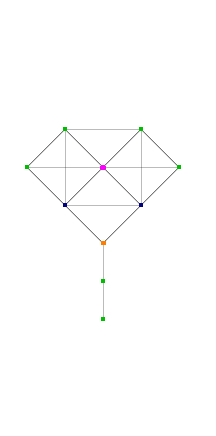
\includegraphics[angle=90,origin=c]{/home/alex/Scrivania/desktop/Tesi/Capitoli/kite}

\caption{Kite graph. The pink node has the highest degree, the orange node
has the highest betweenness and the blue nodes have the highest closeness.
Green nodes are the remaining nodes.}

\end{figure}

To the author's knowledge, there are no previous works trying to apply
the use of centrality measures to enhance the coordination of a team
of robots and due to the variability depending on the centrality measure
used, in this work both closeness and betweenness have been tested.
In the following sections, they are formally introduced with the reasons
for their use.

\subsection{Closeness}

The closeness centrality of a node is defined as the reciprocal of
the sum of the length of the shortest paths between the node and all
the other nodes in the graph \cite{Freeman1978}. This definition
is strongly dependent on the number of nodes $N$ in the graph, thus
closeness is usually normalized by dividing for $N-1$. In this way,
closeness can be defined as the reciprocal of the average distance
between the node and all the other nodes and allows to compare its
value for graphs of different sizes. 

Formally, let $x$ and $y$ be nodes of the graph, and let $d$ be
a real-valued function which provides the length of the shortest path
connecting two nodes, then the normalized closeness value $C\left(x\right)$
is defined as 
\[
C\left(x\right)=\frac{N-1}{\sum_{y\neq x}d\left(x,y\right)}
\]

with $N$ the total number of nodes in the graph, as defined above. 

The original formulation of closeness centrality considers only unweighted
graphs, but it has been extended to be applied also to weighted ones.
The formal definition is the same assuming an appropriate modification
in the implementation of the distance function $d$. Indeed, in an
unweighted graph, it simply has to count the number of edges along
the shortest path linking the two nodes in input, while on a weighted
graph the cost of traversing an edge is proportional to its weight
and thus it has to be included accordingly \cite{Newman2001}.
In the latter case, the distance function $d$ is $d\left(x,y\right)=\sum_{e\in E}w\left(e\right)$,
where $x$ and $y$ are nodes of the graph, $E$ is the set of edges
of the graph composing the shortest path from $x$ to $y$, and $w$
is a real-valued function returning the weight of the edge. 

Closeness tends to consider central nodes the ones in which distance
from all the other nodes is lower on average. Therefore, going back
to an exploration context, placing an agent in the location corresponding
to the highest closeness node makes it possible to reach an assigned
position, not known before, in an expected time lower than any other
starting location with a lower closeness. This reasoning has been
applied to the idle set, which placed in the node with the highest
closeness is likely to already be in a good spot when turned into
active. 

In Figure 3 an example of the distribution of high closeness nodes
is shown for each kind of graph. For the sake of the example, as high
closeness nodes are considered nodes with a value of closeness higher
than the 75\% of the max value. It is interesting to point out how
these nodes are distributed mostly on one corner of the central space
for the topological graph, while they wrap the central obstacle in
the visibility case. Despite the marked differences in their structures
and the number and disposition of high closeness nodes, it is remarkable
that the distance among the highest closeness nodes is really low. 

\begin{figure}
\subfloat[Topological graph. Green dots are the nodes with a value of closeness
lower than the 75\% of the max value.]{\includegraphics[scale=0.4]{\string"/home/alex/Scrivania/desktop/Tesi/Documenti/Marco Catteneo/MRESim/logs/disegni/d3t c\string".eps}

}

\subfloat[Visibility graph. Green dots are the remaining pose nodes and red
ones are the frontier nodes.]{\includegraphics[scale=0.4]{\string"/home/alex/Scrivania/desktop/Tesi/Documenti/Marco Catteneo/MRESim/logs/disegni/d3v c\string".eps}

}

\caption{Distribution of nodes with a closeness higher than the 75\% of the
max value for the topological and the visibility graphs. Blue dots
are the highest closeness nodes, cyan dots are the ones with a high
value of closeness but not the maximum, and edges are omitted for
clarity.}

\end{figure}


\subsection{Betweenness}

Betweenness centrality for a certain node of the graph measures how
much of the total number of shortest paths between other nodes passes
through that node \cite{Freeman1978}. Let $s$, $v$, and
$t$ be three nodes in a connected graph, $\sigma_{st}$ be the total
number of shortest paths connecting $s$ and $t$ and $\sigma_{st}\left(v\right)$
be the number of those paths which go through $v$, then the betweenness
$B\left(v\right)$ for the node $v$ is defined as 
\[
B\left(v\right)=\sum_{s\neq v\neq t}\frac{\sigma_{st}\left(v\right)}{\sigma_{st}}
\]

where the sum is performed over each pair of nodes in the graph. The
graph needs to be connected, otherwise, each $\sigma_{st}$ where
$s$ or $t$ is a disconnected node would result in a division by
zero. However, this is always granted in the context of this work
because of the way in which graphs are built. 

Betweenness followed an evolution similar to the one of closeness,
being at first defined on unweighted graphs \cite{Freeman1978}
and then extended to the case of weighted ones \cite{Newman2001}.
In the case of weighted graphs, weights impact how shortest paths
are computed, making necessary the use of algorithms like Dijkstra's
or Breadth-First Search to deal with them. Once the shortest paths
are provided, the algorithm to compute the betweenness is the same.
Similarly to closeness, where the introduction of weights on the edges
only affects the computation of the distances between nodes. 

The idea behind this metric is to assign higher importance to the
nodes which are along more shortest paths linking couples of other
nodes. In different works about social networks analysis \cite{Freeman1978},
betweenness is used to find out which are the nodes having more control
over the information flow. Nodes with a high value of betweenness
are along more shortest paths, thus more information goes through
them and an eventual disconnection may cause loss of information or
a separation of the graph into two sub-graphs. However, a node of
this kind is likely to be fundamental for what concerns the connectivity
of the graph, differently from a node with low betweenness. According
to this, the approach based on betweenness has been conceived. Being
interested in an effective positioning of the idle set, a location
with a high value of betweenness is an ideal candidate because it
guarantees to be a crucial point for the connectivity of the environment
and when the idle set is turned into active, it is likely to be in
a good position to navigate towards the assigned frontier. 

In Figure 4, the nodes with high betweenness are plotted over the
representation of the graphs provided before. The first thing that
catches the eye is the difference in the number of this kind of nodes
between the topological and the visibility graphs, being a lot more
in the first one. This can be justified by considering the reduced
size of the graph in that case, which makes every node on more shortest
paths, thus with a higher value of betweenness. Also for this metric
holds what stated previously about the highest closeness node. Despite
the different structures of the two graphs and the even more marked
difference in the distribution of high betweenness nodes, the highest
values of the metric are measured in two extremely near locations.
This enforces the idea that these metrics can characterize the environment
mapped and by an analysis of them, it might be even possible to discriminate
among different types of it. 

\begin{figure}
\subfloat[Topological graph. Green dots are the nodes with a value of betweenness
lower than the 50\% of the max value.]{\includegraphics[scale=0.4]{\string"/home/alex/Scrivania/desktop/Tesi/Documenti/Marco Catteneo/MRESim/logs/disegni/d3t b\string".eps}

}

\subfloat[Visibility graph. Green dots are the remaining pose nodes and red
ones are the frontier nodes.]{\includegraphics[scale=0.4]{\string"/home/alex/Scrivania/desktop/Tesi/Documenti/Marco Catteneo/MRESim/logs/disegni/d3v b\string".eps}

}

\caption{Graphs with nodes having a high value of betweenness highlighted.
Orange nodes are the ones with the highest betweenness, while in yellow
nodes with a betweenness comprised between the 50\% and the max value
are drawn. Edges are omitted for clarity.}

\end{figure}


\section{Comparative metrics}

The different methods proposed are compared based both on practical
measures, as the time taken to fulfill the termination criterion and
the distance traveled by the robots, and on theory-based measures,
namely interference among robots and their availability. 

The use of time and distance traveled as comparison metrics is intuitive
if looking at some of the application contexts. Teams of robots are
often used in search and rescue scenarios, where the time needed to
complete the exploration is a fundamental aspect to take into account.
Thus, a faster approach is overall preferable to a slower one in such
a scenario. The distance traveled is a less important factor in discriminating
among different mechanisms, but it may provide an interesting and
more complete overview of an approach compared to others. 

In the simulations run in this work, the termination criterion used
is the exploration of the 95\% of the environment. At the end of each
run, the number of discrete time steps taken and the average distance
traveled by the robots are stored and then compared during the analysis
of the results. The decision of considering the number of time steps
rather than the time taken by the exploration has been carried on
to exclude machine-dependent aspects from the results. Some of the
mechanisms implemented are way more computationally intensive than
the ones based on the barycenter computation, and comparing their
results on the effective time taken would have been faked by the computing
capability of the machine running simulations. 

These two metrics have been considered sufficient to characterize
from a practical point of view each mechanism analyzed. Nevertheless,
two further measures are used to examine the mechanisms, which are
named interference and availability. They are at first introduced
in \cite{Rogers2013} and formalized in \cite{Cattaneo2017}. 

\subsection{Interference }

Interference quantifies the average distance held by agents during
the exploration and the higher the distance, the lower the value.
A high value of interference is desirable because as the average distance
among robots increases, it reduces the possibility of incidents and
the complexity in the management of the system. Moreover, it is also
an indirect measure of how parallel the exploration is being carried
on because it increases as the robots are spread on the environment.
According to this, the value of interference for a particular coordination
mechanism can provide useful information about the amount of parallelizability
exploited as compared to other mechanisms.

The value of interference $\lambda$ for an agent $a$ is computed
at each step $t$ of the exploration by calculating the average distance
between $a$ and all the other agents $a'$ in the team $A$, thus
it can be formally written as 
\[
\lambda_{t}\left(a\right)=\frac{1}{N-1}\sum_{a'\in A|a'\neq a}d\left(P_{t}\left(a\right),P_{t}\left(a'\right)\right)
\]

where $N$ is the size of the team, $P_{t}$ is a function providing
the position of an agent at time $t$, while $d$ is the function
that computes the distance between two positions of the environment. 

This definition only relates to one agent at a particular instant
of the exploration. To completely characterize the value of interference
for the whole exploration, it needs to be at first generalized over
the set of agents composing the team and then over the entire time
needed to complete the exploration. In this way, its value computed
for a specific coordination mechanism is comparable with the ones
provided by other mechanisms over the same exploration problem. 

The first generalization consists in extending the definition of interference
to all the robots in the team, rather than considering only a single
robot, and this is simply done by averaging the values of interference
of each agent:
\[
\lambda_{t}=\frac{1}{N}\sum_{a\in A}\lambda_{t}\left(a\right)
\]

At this point, it is possible to integrate this expression over the
entire time taken by the exploration, which is considered to take
values in $\left[0,\ldots,t_{T}\right]$ with $t_{T}$ being the time
step of the fulfillment of the termination criterion $T$. The definition
of the interference for the coordination mechanism applied to a specific
instance of the exploration problem considered is 
\[
\lambda=\frac{1}{t_{T}+1}\sum_{t=0}^{t_{T}}\lambda_{t}
\]

This states that the interference for the whole exploration can be
computed by averaging over the total time taken the values of interference
for the team. In this way, the value of interference obtained can
be exploited to compare different coordination mechanisms, avoiding
that differences in the duration of the exploration impact on this
measure. 

\subsection{Availability}

Availability is a measure of the distance between an agent and its
assigned location. It can be formally defined at first for a single
agent $a$ in a certain time step $t$ as 
\[
\alpha_{t}\left(a\right)=d\left(P_{t}\left(a\right),G_{t}\left(a\right)\right)
\]

where $\alpha$ is the symbol used for the availability and $G_{t}$
is a function returning the location of the frontier assigned to the
agent in input. The two auxiliary functions $d$ and $P_{t}$ are
the same presented in the previous section to define the interference. 

Similarly to what done for the interference, this definition can be
generalized to the whole team and the whole exploration. Following
similar reasoning and with the same meaning of the symbols, the availability
for the whole team at a certain instant $t$ of the exploration is
\[
\alpha_{t}=\frac{1}{N}\sum_{a\in A}\alpha_{t}\left(a\right)
\]

recalling that $A$ is the set of agents composing the team and $N$
is its cardinality. Averaging this result over the whole exploration
time $t_{T}$ defines availability for a coordination mechanism applied
to a specific instance of the exploration problem, thus it turns out
to be 
\[
\alpha=\frac{1}{t_{T}+1}\sum_{t=0}^{t_{T}}\alpha_{t}
\]

This value of the availability is independent of the time taken to
meet the termination criterion and therefore, allows a comparison
among different coordination mechanisms, without being affected by
their respective performance in terms of time. It is important to
highlight how availability has the opposite trend of interference.
Indeed, a mechanism with low availability assigns robots to locations
near their positions, which makes the agents update the environment
more frequently than a scenario in which robots have to travel a long
distance before scanning unknown portions of it. 

This metric has a two-fold interpretation. From one side, it shows
whether a mechanism assigns robots to far or close targets. On the
other side, it can provide insights on the effectiveness of the proactivity
when comparing two mechanisms which differ only in this aspect. This,
in particular, is the setting of this thesis. The differences of the
mechanisms analyzed concerns only the proactive allocation of the
idle set, and thus a mechanism that has a lower value of availability
is likely to place this set of robots in a position nearer to the
frontiers. Strong evidence of this relation between proactivity and
availability is provided by \cite{Cattaneo2017} in the comparison between
reserve and proactive reserve, where by moving the idle set towards
the barycenter of locations of the active agents, the latter method
ensures agents to travel a shorter distance once turned into active
with respect to the former one.

It is worth to point out also that the absolute value of both this
metric and the interference is highly affected by the particular configuration
of the environment explored and by the team size, for this reason,
comparisons among mechanisms based on them do make sense only if done
on the same instance of exploration problem. 
\begin{thebibliography}{1}
\bibliographystyle{plain}
\bibliography{/home/alex/Scrivania/desktop/Tesi/Capitoli/Bibtex}
\end{thebibliography}

\end{document}
